%****************************************************************
% Chapter X
%****************************************************************
\label{chapter-technology}
\chapter{Technology}

****************************************************************\\%####
How am I going to discover it?\\
.... why is best suited to my aims, because …\\

%****************************************************************
\section{Android Phone}

****************************************************************\\%####

%****************************************************************
\subsection{Mobile Device}

****************************************************************\\%####
Sensor\\

%****************************************************************
\subsection{Google Cardboard}

****************************************************************\\%####
Google VR SDK\\

%****************************************************************
\section{OpenGL ES}

****************************************************************\\%####
OpenGL ES 2.0, 3.0,  3.1, 3.1 ext\\

%****************************************************************
\section{Keyhole Markup Language}

We were looking for a simple markup languages that we can publish and consume data  in interoperable formats without the need for technical assistance.

In this section, we present Keyhole Markup Language (KML) \parencite{Google.kml.2016}, a file format to display geographic data ( (Note that KML files can be combined with other supporting files such as imagery in a zip archive, producing a KMZ file). It is an international standard maintained by the Open Geospatial Consortium, Inc. (OGC), and also it is supported by many Virtual Globes (VG) applications and other GIS systems and is therefore already becoming a de facto standard. Such as the most wellknown VG application Google Earth that has the largest community, NASA World Wind has more focus toward scientific users, and ArcGIS Explorer that is a lightweight client to the ArcGIS Server \parencite{blower.sharing-visualizing.2007}.

From an environmental science point of view, KML is a somewhat limited language. It describes only simple geometric shapes on the globe (points, lines and polygons) and is not extensible. It is, in many respects, analogous to Geography Markup Language (GML) 3.0+ is much more sophisticated and allows the rich description of geospatial features such as weather fronts and radiosonde profiles. So, KML is currently not suitable as a fully-featured, general-purpose environmental data exchange format.

Figure \ref{fig:kml-schema} shows the KML schema. From the point of view of usability, KML spans a gap between very simple (e.g. GeoRSS) and more complex (GML) formats, that makes it easy for non-technical scientists to share and visualize simple geospatial information which can then be manipulated in other applications if required. Also it makes it easier for user to visualize their data quickly using a single, simple data file. Moreover, its rapidly-growing adoption by scientists, and it is important to be aware of that virtual geographic data visualization (and KML) do not attempt to replace more sophisticated systems. 

\begin{figure}[H]
\caption[kml-schema]{KML schema \parencite{Google.kml.2016}}
\label{fig:kml-schema}
\centering
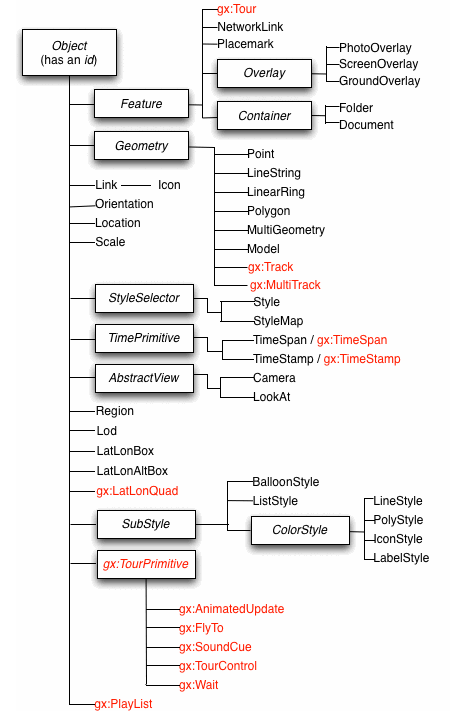
\includegraphics[height=0.5\textheight]{Figures/kml-schema.png}
\decoRule
\end{figure}

%****************************************************************
\section{Network Data}

****************************************************************\\%####
File server - golang\\
Client - volley, Jsoup\\

%****************************************************************
